\section{问题一求解与分析}
\label{sec:q1}
\subsection{问题的描述与分析}
每个子图均作为一个独立执行任务。子图划得过细，虽然容易将计算量分散到多个核心，却增加了任务切换和跨子图搬运；子图过大，又可能压低并行度，并加剧片上存储压力。因此，子图划分、核心归属和核内子图顺序应联合决定。本文用一个完整方案描述三项决策，再以固定执行规则得到总体任务执行时间。后两问保持这一决策空间，通过改变任务边界、交接和缓存规则，解释同一类方案的执行差异。

图~\ref{fig:q1_overview} 概括本问的求解逻辑。先从原始计算图提取依赖、计算负载和张量复用关系，形成若干完整初始方案；再围绕当前可行方案进行互补的邻域改进。计算开销较低的结构预检和下界用于筛选候选，完整执行评价决定是否保留候选。最后从核数扩展、逐例差异、搜索过程和目标界四个方面分析结果。
\begin{figure}[htbp]
\centering
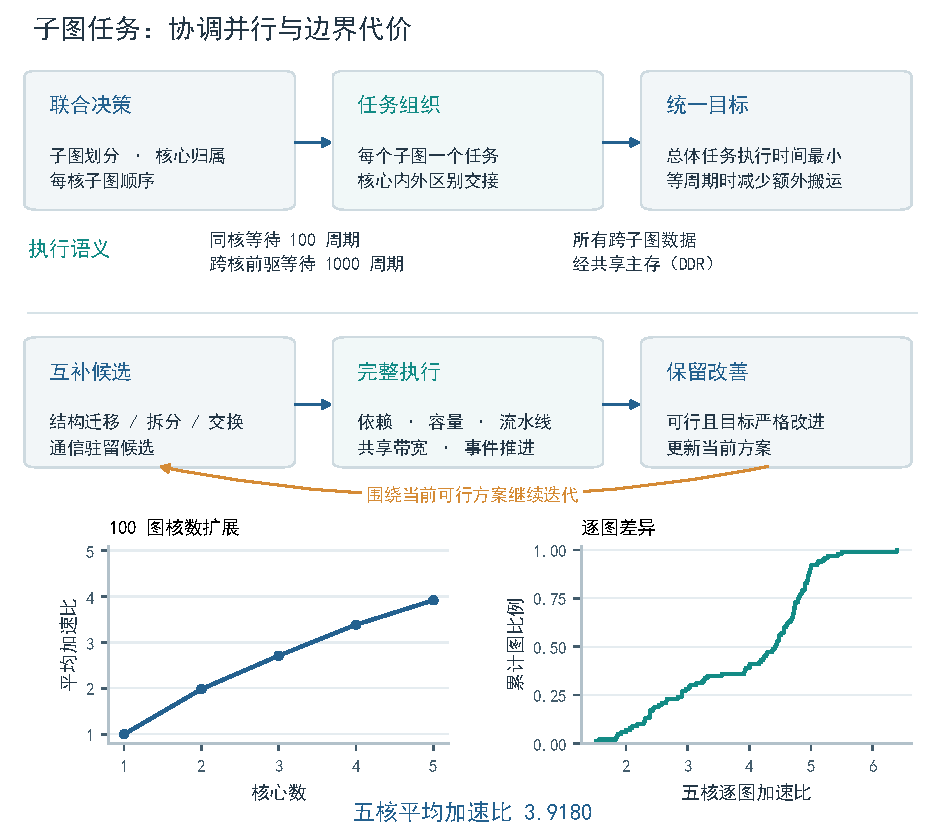
\includegraphics[width=\textwidth]{../求解/问题一/图片/q1_overview.pdf}
\caption{问题一的联合建模与迭代改进框架}\label{fig:q1_overview}
\end{figure}


\subsection{联合决策模型与统一目标}
\subsubsection{计算图、张量与划分}
原始二部有向无环图记为 $G=(T\cup O,E)$，其中 $T$ 为张量集合，$O$ 为操作集合。定义需要分配的非边界搬运算子集合
\begin{equation}
 V=\{o\in O:\operatorname{type}(o)\notin\{\mathrm{COPY\_IN},\mathrm{COPY\_OUT}\}\},
\end{equation}
\noindent 式中，$\operatorname{type}(o)$ 为操作类型，$\mathrm{COPY\_IN}$ 和 $\mathrm{COPY\_OUT}$ 分别表示核外数据搬入与搬出。模型保留原始算子的类型与计算周期、张量大小和依赖关系，再按任务划分及执行规则重建边界搬运操作。对于张量 $t\in T$，记其大小为 $b_t$，生产者与消费者集合分别为 $P_t$ 和 $C_t$。同一张量的多个消费者共享其生产关系，因而具有潜在的数据复用机会。生产者到多个消费者的关系可用有向超边表达；相关无环超图划分研究提供了这种集合表示\cite{A39}。本文仍依据任务边界生成实际搬运，候选中的通信排序量按相关张量字节构造，不以超边连接度替代实际搬运量。

设可用核心集合为 $K=\{1,\ldots,n\}$。完整方案写为
\begin{equation}
 x=(\mathcal P,a,\boldsymbol\pi),\qquad
 \mathcal P=(V_1,\ldots,V_m),\quad a:\{1,\ldots,m\}\longrightarrow K ,
 \label{eq:plan}
\end{equation}
\noindent 式中，$m$ 为子图数，$\boldsymbol\pi=(\pi_1,\ldots,\pi_n)$；$V_i$ 是第 $i$ 个子图包含的算子集合，$a(i)$ 是该子图的核心归属，$\pi_k$ 是核心 $k$ 上子图的执行顺序。划分满足
\begin{equation}
 V_i\ne\varnothing,\qquad \bigcup_{i=1}^{m}V_i=V,\qquad
 V_i\cap V_j=\varnothing\quad(i\ne j).
 \label{eq:partition}
\end{equation}
每个子图恰好出现于一个核心序列且只出现一次，允许部分核心没有子图。核数增大扩展了可用资源和方案选择空间，具体使用的核心数由方案决定。

将各 $V_i$ 收缩为顶点，可得到子图依赖商图 $H(\mathcal P)$。再加入各 $\pi_k$ 中相邻子图的顺序边，得到 $H_x$。必要条件为
\begin{equation}
 H_x\text{ 是有向无环图}.
 \label{eq:acyclic}
\end{equation}
无环性需要在收缩后重新检查。例如，交错地收集依赖链上不连续的算子，可能在商图中产生双向依赖。无环划分文献对此给出了明确约束\cite{A02}。执行中还存在执行流水线和存储复用关系，所以式~\eqref{eq:acyclic} 用于结构筛选，最终可行性由完整执行确定。

\subsubsection{执行映射与三问的共同方案空间}
记固定配置为 $\theta$，问题编号为 $q\in\{1,2,3\}$。定义执行映射
\begin{equation}
 \mathcal E_q(G,x;\theta)
 =\bigl(\operatorname{feas}_q(x),\mathcal R_q(x),C_q(x),D_q(x)\bigr),
 \label{eq:evaluator}
\end{equation}
\noindent 式中，$\operatorname{feas}_q(x)\in\{0,1\}$ 表示可行性，$\mathcal R_q(x)$ 为完整执行事件序列，$C_q(x)$ 为总体任务执行时间，$D_q(x)$ 为总额外数据搬运量（额外COPY字节）。对于重建边界搬运、插入存储换出和取回后得到的操作集合 $J_q(x)$，设操作 $j$ 的开始、完成时刻为 $s_j,f_j$。定义
\begin{equation}
 C_q(x)=\max_{j\in J_q(x)} f_j,
 \qquad x\in\mathcal F_q:=\{x:\operatorname{feas}_q(x)=1\},
 \label{eq:makespan}
\end{equation}
\noindent 式中，$\mathcal F_q$ 为完整执行可行的方案集合，$C_q$ 以时钟周期计，$D_q$ 以字节计。本文以 $C_q$ 为主目标，周期相同则选择 $D_q$ 较小者，即
\begin{equation}
 \min_{x\in\mathcal F_q}^{\mathrm{lex}}\bigl(C_q(x),D_q(x)\bigr),
 \label{eq:objective}
\end{equation}
\noindent 式中，$\mathrm{lex}$ 表示字典序比较。总额外数据搬运量等于调度后逻辑COPY总字节减去原图已有COPY字节，包含重建边界搬运与缓存换入换出。若读请求命中L2，则改由L2服务，但仍保留相应逻辑COPY操作；实际DDR服务字节另按请求的服务路径统计。

三问均采用式~\eqref{eq:plan} 的决策，改变的是执行映射。记算子 $v$ 所属子图为 $g(v)$，其执行任务标识为
\begin{equation}
 \chi_q(v)=\begin{cases}g(v),&q=1,\\a(g(v)),&q=2,3.\end{cases}
 \label{eq:task}
\end{equation}
这一定义把三问组织为同一模型的三个执行场景：第一问任务随子图划分，第二问任务随核心划分，第三问在第二问基础上增加共享只读缓存。三项决策通过各自的执行规则共同影响同一个优化目标。

\subsection{第一问的执行、存储与带宽约束}
\subsubsection{任务边界与交接}
一个子图对应一个Task。同一核心相邻任务之间也需要把边界张量写入 DDR，下一任务再读取，因此同核任务边界也产生搬运代价。任务聚类研究中的分组思想\cite{A49}需在这一边界条件下使用。图~\ref{fig:q1_task} 表示第一问的任务边界与就绪关系。
\begin{figure}[htbp]\centering
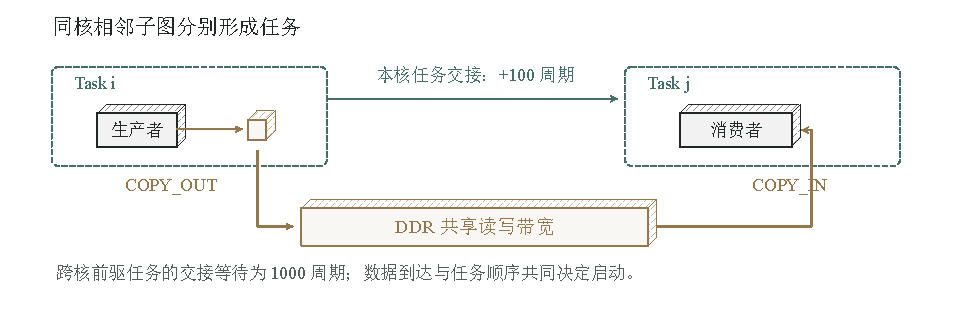
\includegraphics[width=\textwidth]{../求解/问题一/图片/q1_task.pdf}
\caption{子图级任务的边界与交接}\label{fig:q1_task}
\end{figure}

设任务 $i$ 的启动、完成时刻分别为 $S_i$ 和 $F_i$。任务 $j$ 的启动须同时满足其数据依赖和本核前序任务约束。对相邻本核任务，须有 $S_j\ge F_i+100$；对跨核前驱任务，须有 $S_j\ge F_i+1000$。存在多个前驱时，启动时刻受这些约束的最大值限制。100 与 1000 均以周期计，搬运本身占用的共享 DDR 服务时间还需单独通过事件执行获得。

任务边界使粒度选择出现双重影响。合并子图可以消除两者之间的一部分任务切换和边界搬运，但也固定了更多算子的共同归核，减少跨核重叠机会。进一步合并还可能延长张量驻留区间，引发自动换出。粒度选择因而需要同时考虑边界搬运、计算并行与容量压力。

\subsubsection{固定核内调度与片上容量}
每核具有矩阵、向量、读入和写出四条流水线（Pipe）。每条流水线同时至多服务一个操作；不同流水线可以在满足依赖和容量条件时重叠。算子的开始时刻满足前驱完成、所属流水线可用以及所需片上缓冲可分配等条件。固定核内处理先给出固定操作顺序，再处理存储换出，最后生成流水线依赖。本文的决策作用于子图划分、归核和核内子图顺序。

令 $r\in\{\mathrm{L1},\mathrm{UB}\}$ 表示片上存储区，$B_r$ 为容量；$\mathcal B_{k,r}(\xi)$ 是执行时刻 $\xi$（周期）核心 $k$ 在该区已分配且尚未释放的缓冲实例集合。容量条件写为
\begin{equation}
 \sum_{b\in\mathcal B_{k,r}(\xi)}\operatorname{size}(b)\le B_r,
 \quad B_{\mathrm{L1}}=524288\ \mathrm B,\quad B_{\mathrm{UB}}=131072\ \mathrm B,
 \label{eq:capacity}
\end{equation}
\noindent 式中，$\operatorname{size}(b)$ 为缓冲实例 $b$ 占用的字节数。一个逻辑张量在不同核上的驻留副本分别占用相应核心的容量。任务切换还会清除本核任务私有存储，跨任务复用必须经由规定路径完成。

在固定顺序下容量不足时，执行规则依据下一次使用位置选择允许换出的张量，并在后续需要时重新取回。当前操作需要的输入、输出等对象受换出资格限制。换出与取回属于执行映射；调整划分和顺序可能改变其发生位置及搬运量。联合调度与存储优化研究揭示了驻留状态与片外访问之间的联系\cite{A16}。本文据此分析活跃集和驻留压力，在固定分配与换出规则下提出划分和顺序候选。

\subsubsection{共享 DDR 的事件推进}
设 DDR 总带宽为 $\beta_{\mathrm{DDR}}=60\ \mathrm B/\text{周期}$。对当前在途 DDR 读写请求集合 $\mathcal A_D(\xi)$，记 $m_D(\xi)=|\mathcal A_D(\xi)|$。若以独占该带宽所需周期表示请求 $j$ 的剩余服务量 $w_j$，在没有新的发射或完成事件的时间区间内，有
\begin{equation}
 w_j(\xi+\Delta)=\max\left\{0,w_j(\xi)-\frac{\Delta}{m_D(\xi)}\right\},\quad j\in\mathcal A_D(\xi),
 \label{eq:bandwidth}
\end{equation}
\noindent 式中，$\Delta$ 为在途集合不变的事件间隔，$m_D(\xi)>0$；$w_j$ 与 $\Delta$ 均以周期计。请求初始独占服务量按字节数除以带宽向上取整，且至少为1周期。新的读写发射、请求完成和任务就绪都会改变下一个事件时刻。事件执行依次处理完成事件，释放依赖和存储，再发射满足条件的新操作。

改变子图边界或归核即使减少了搬运字节，也可能使请求更集中，从而延迟关键计算链。第4.5节给出各来源的内部排序量；所有候选的正式周期均按上述事件过程计算。

\subsection{下界、候选过滤与质量界}
\subsubsection{对全体方案有效的下界}
取所有可行方案都保留的计算依赖图 $G_c$，其中算子 $v$ 的固定服务周期为 $p_v$，计算流水线类型为 $\rho(v)$。定义计算路径、流水线负载和必要 DDR 流量下界：
\begin{align}
 L_{\mathrm{path}}&=\max_{P\text{ 为 }G_c\text{ 中依赖路径}}\sum_{v\in P}p_v,\\
 L_{\mathrm{load}}&=\max_r\frac{\sum_{v:\rho(v)=r}p_v}{n},\\
 L_{\mathrm{DDR}}&=\frac{B_{\mathrm{mandatory}}}{\beta_{\mathrm{DDR}}},\qquad
 L=\max\{L_{\mathrm{path}},L_{\mathrm{load}},L_{\mathrm{DDR}}\},
 \label{eq:lower}
\end{align}
\noindent 式中，$r$ 遍历计算流水线类型，$B_{\mathrm{mandatory}}$ 只包含能证明所有方案都必须通过 DDR 服务的字节。对第一、二问，初始输入读取和最终输出写出提供这种必要流量；第三问的初始缓存为空，无逻辑别名时首次读取仍须经过 DDR。存在显式逻辑别名时，第三问的流量下界仅计必要写出量。

\textbf{命题1：}在计算依赖保留、算子不重算或删除、同类计算流水线每核串行、必要 DDR 流量判断成立的条件下，对任意可行方案 $x$，有 $L\le C_q(x)$。

\textbf{证明：}同一计算依赖路径上的算子只能依次完成，故执行周期不小于任意路径的计算服务量之和。每种计算流水线在 $n$ 个核心上的总能力为每周期至多提供 $n$ 个流水线周期，因此其总工作量除以 $n$ 不大于执行周期。DDR 在任意长为 $C_q(x)$ 的区间内至多服务 $\beta_{\mathrm{DDR}} C_q(x)$ 字节，必要流量又给出第三项约束。三项分别给出有效下界，取最大值仍成立；计算与搬运可以重叠，因此这里不将三项相加。证毕。

\subsubsection{固定候选的下界}
固定完整候选 $x$ 后，归核已经确定，可进一步计算每个核心各类流水线的工作量下界。第一问还可以在任务依赖和核心顺序合图上，按每个任务的计算负载下界及对应交接等待递推最早完成下界。设任务 $i$ 的工作下界为 $\ell_i$，前驱集合为 $\operatorname{pred}_x(i)$，交接等待为 $d_{hi}$，则
\begin{equation}
 z_i=\ell_i+\max_{h\in\operatorname{pred}_x(i)}(z_h+d_{hi}),
 \label{eq:taskbound}
\end{equation}
\noindent 式中，$z_i$ 为任务 $i$ 的完成时刻下界；无前驱时最大项取零。$\ell_i$ 取该任务各计算流水线总负载的最大值，允许流水线充分重叠；$d_{hi}$ 只使用规定的任务等待。由拓扑序归纳可知，真实任务完成时刻不早于 $z_i$。把这些项以及固定任务边界产生的必要搬运下界取最大值，得到候选专属下界 $L(x)$。

\textbf{命题2：}若 $L(x)\le C_q(x)$，当前已保留方案周期为 $U$，则 $L(x)>U$ 的候选不能改善主目标。

\textbf{证明：}$C_q(x)\ge L(x)>U$，故该候选的周期严格更差。证毕。过滤使用严格大于；当 $L(x)=U$ 时，候选仍可能在相同周期下减少额外 COPY 字节。候选下界刻画固定 $x$ 的周期约束；全局质量界使用对全部方案成立的 $L$。

\subsubsection{可行上界与相对差距}
令 $C_q^*$ 为全局最优周期，当前可行周期为 $U$。当 $0<L\le C_q^*\le U$ 时，
\begin{equation}
 0\le\frac{U-C_q^*}{U}\le1-\frac{L}{U},\qquad
 0\le\frac{U}{C_q^*}-1\le\frac{U}{L}-1,
 \label{eq:gap}
\end{equation}
\noindent 式中，第一组不等式以当前周期为分母，量化仍可能减少的比例；第二组不等式以最优周期为分母，量化当前解的相对超额。本文以第一式右侧作为近界停止依据，当其不超过 $0.0025$ 时停止继续改进。其他停止条件见算法~\ref{alg:joint}。

\subsection{多邻域迭代改进算法}
\subsubsection{初始构造与当前可行方案}
已有同配置方案经有效执行结果确认后可作为初值；否则由下述构造产生候选。构造时取 $\widetilde p_v=\max\{1,p_v\}$，设 $w_r(A)=\sum_{v\in A:\rho(v)=r}\widetilde p_v$，$W(A)=\max_r w_r(A)$。从算子依赖图的弱连通分量出发，依次切分负载最大的分量。对固定拓扑序的非空前缀 $A$ 和后缀 $B$，切点按
\begin{equation}
 \min_{A\dot\cup B=V_i}
 \left[\max\{W(A),W(B)\}+\gamma_q F(A,B)/\beta_{\mathrm{DDR}}\right],
 \quad \gamma_1=2,\quad\gamma_2=\gamma_3=1,
 \label{eq:frontier_construct}
\end{equation}
\noindent 式中，$F(A,B)$ 是在两侧均有生产或消费操作的张量字节总和；每个张量只计一次。该量用于切点排序，不是总额外数据搬运量。长度大于6时只考察位置比例为15\%--85\%的切点；并列时先取负载差较小者，再取较早切点。切开后分别取两侧弱连通分量。对粒度 $g\in\{2,4,8\}$，当最大块负载不超过 $\max\{1,W(V)/(gn)\}$ 或已切分 $2gn$ 次时结束该构造。

给定划分后，以算子上行优先级 $r_v=\widetilde p_v+\max_{u\in\operatorname{succ}(v)}r_u$（无后继时最大项为0）的块内最大值，在就绪子图中选取优先级最高者。对待放置子图 $i$，计算各核的估计完成位置
\begin{equation}
 \widehat E_i(k)=\max_r\{\max(\ell_{k,r},R_i(k))+w_r(V_i)\},\qquad
 a(i)=\mathop{\arg\min}_{k\in K}^{\mathrm{lex}}
 \left(\widehat E_i(k)+\frac{Q_i(k)}{4\beta_{\mathrm{DDR}}},\max_r\ell_{k,r},k\right),
 \label{eq:construct_map}
\end{equation}
\noindent 式中，$\ell_{k,r}$ 为已安排子图在核 $k$、流水线 $r$ 上的估计负载位置；$R_i(k)$ 为前驱估计完成时刻加交接等待后的最大值，空前驱取0。交接等待在第一问取同核100、跨核1000周期，在后两问取同核0、跨核500周期。$Q_i(k)$ 为子图外部输入字节：第一问全部计入，后两问扣除此前已给核 $k$ 分配过的输入张量。选中核心后将 $i$ 接至其序列末端；对 $w_r(V_i)>0$ 的流水线，令 $\ell_{k,r}\leftarrow\max\{\ell_{k,r},\widehat E_i(k)-W(V_i)\}+w_r(V_i)$，其余不变。

式~\eqref{eq:construct_map} 是上行优先级与最早完成时间（Earliest Finish Time，EFT）思想下的构造估计\cite{A01}，不等于共享带宽执行周期。还保留单前驱、单后继边连接的链分组，以及按依赖层宽度变化划分阶段的构造；同阶段同核心的块可合并。基础来源同时探索不同阶段粒度，结构来源探索链分组在不同有效核数和通信权重下的映射。分组与并行执行共同决定候选价值\cite{A08}，所有初值均用 $\mathcal E_q$ 确认。

\subsubsection{互补候选与完整方案更新}
记基础、结构、驻留和缓存时序来源分别为 $\mathrm B,\mathrm S,\mathrm M,\mathrm F$。基础候选 $\mathcal N_{\mathrm B}$ 包括前述多粒度构造，以及负载驱动的迁移、前沿切分和同核相邻子图交换。其部分候选按
\begin{equation}
 \widehat C_q(y)=\max\{\widehat C_{\rm time}(y),\widehat C_{\rm bus}(y)\}
       +\widehat D_{\rm spill}(y)/\beta_{\mathrm{DDR}},
 \label{eq:base_proxy}
\end{equation}
\noindent 式中，$\widehat C_{\rm time}$ 为简化时序估计，$\widehat C_{\rm bus}$ 为估计DDR/L2服务负载的最大值，$\widehat D_{\rm spill}$ 为活跃区间超容量量导出的换入换出字节估计。它们只用于该来源内排序；共同候选入口使用的是有效下界 $L(y)$，不将式~\eqref{eq:base_proxy} 用于证明性剪枝。

结构候选 $\mathcal N_{\mathrm S}$ 包含四种变换。取当前合图 $H_x$ 的拓扑序 $\sigma$，用 $\sigma|_A$ 表示只保留集合 $A$ 中子图的子序列。对选定子图集合 $A$ 及新归核 $\mu:A\to K$，定义
\begin{equation}
 a'(i)=\begin{cases}\mu(i),&i\in A,\\a(i),&i\notin A,\end{cases}
 \qquad \pi'_k=\sigma|_{\{i:a'(i)=k\}},\qquad
 y=(\mathcal P,a',\boldsymbol\pi'),
 \label{eq:group_move}
\end{equation}
\noindent 式中，$A=\{i\}$ 给出单子图迁移；$A=\{i,j\}$ 且互换两者归核给出跨核交换；令两者归至同一核给出联合迁移。前缀拆分则把 $V_i$ 的拓扑序在 $1/4,1/2,3/4$ 处截为两个非空块，保留前块归核，将后块放到负载较轻的另一核，再按 $\sigma$ 重建核序。大划分优先考察晚完成、高负载和高跨核通信子图；迁移组合按最大流水线负载变化加关联跨核字节变化除以DDR带宽排序。该关联字节量同样不是正式COPY指标。

驻留候选 $\mathcal N_{\mathrm M}$ 根据生产与消费关系重组完整子图。第一问特有的生产者释放切分针对长任务：对跨核张量 $t$ 在 $V_i$ 内的生产者，取其组内前驱闭包 $A$，令 $B=V_i\setminus A$。当两部分非空且
\begin{equation}
 F_i-\max_{v\in P_t\cap V_i}f_v>100,
 \label{eq:release_split}
\end{equation}
\noindent 式中，$F_i$、$f_v$ 分别是当前执行中任务与生产者的完成时刻。满足式~\eqref{eq:release_split} 时，将 $(A,B)$ 依次留在原核。按此时间差递减取至多4个候选，尝试提前释放跨核数据，同时仍须支付新增任务交接成本。后两问的驻留重组见算法~\ref{alg:residency}，第三问另增加算法~\ref{alg:fifo} 的纯顺序候选。

多初值与局部迁移共同组织搜索\cite{A42}。各来源均给出完整 $y$；在同配置完整评价后，统一更新为
\begin{equation}
 x^+=\begin{cases}
 y,&y\in\mathcal F_q\ \text{且}\ (C_q(y),D_q(y))<_{\rm lex}(C_q(x),D_q(x)),\\
 x,&\text{其他情形}.
 \end{cases}
 \label{eq:accept}
\end{equation}
接受后以 $(x^+,\mathcal R_q(x^+))$ 重建依赖当前解的局部候选；与当前解无关的构造继续给出尚未考察的方案。相同完整方案不重复评价。

\subsubsection{来源选择与有限预算}
候选生成和完整评价的成本差异较大，因此按近期反馈分配搜索机会。对第 $j$ 次调用，记评价前当前最好周期为 $U_j$，候选周期为 $C_j$，周期收益取 $g_j=\max\{0,1-C_j/U_j\}$；评价失败或周期持平时记零。设来源 $s$ 的近期收益均值为 $\bar g_s$，生成与评价总用时中位数为 $\widehat c_s$，失败比例为 $r_s$，已完成调用数为 $N_s$，所有来源的总调用数为 $N_{\rm call}$。在初次覆盖、可用性和剩余时间准入条件满足后，比较指数
\begin{equation}
 I_s=\frac{\bar g_s+0.012\sqrt{\log(2+N_{\rm call})/(1+N_s)}}{
 \max(0.005,\widehat c_s)(1+r_s)},
 \label{eq:sourcepriority}
\end{equation}
\noindent 式中，近期均值、中位数和失败比例按最近八次调用计算。前项奖励已观察到的改进，第二项为尚未充分尝试的来源保留机会，分母计入运行成本和失败倾向。搜索资源根据测量反馈分配的思路与程序自动调优中的经验一致\cite{A12}；式~\eqref{eq:sourcepriority} 将上述因素组合为启发式来源优先级。

初期优先选择已完成调用不足2次且已生成候选不足12个的来源。第三问仅在结构与驻留成功调用合计不足4次、且累计用时低于 $\min\{20,0.18\tau_{\max}\}$ 秒时暂缓缓存时序来源。其后优先选择距上次调用已隔至少8次的来源，否则比较式~\eqref{eq:sourcepriority}；准入成本为 $1.2\max\{0.005,\widehat c_s\}+0.05$ 秒，若已有调用记录且无来源能在剩余时间内完成，则停止。

每个图、问题及核数配置的累计主机时间上限 $\tau_{\max}=600$ 秒，评价上限为2048次；总时间包含解析、已有方案确认、候选生成、评价与保存，第三问的同方案配对在总预算内预留时间。近界、预算耗尽、来源耗尽或停滞均可终止搜索。停滞要求同时满足：至少30秒没有周期改善、连续至少32次评价未改善周期、每个仍可用来源至少8次未改善周期。仅次要指标改善可以接受，但不重置周期停滞条件。

\subsubsection{可行性保持与目标单调性}
\textbf{命题3：}若初始方案 $x^{(0)}\in\mathcal F_q$，每次只在相同配置下接受完整执行可行且字典序严格改善的候选，则所有已保留方案均可行，且目标序列字典序单调不增。

\textbf{证明：}初始方案可行。第 $k$ 步若没有接受新候选，则保留 $x^{(k)}$；若接受 $y$，其已通过完整执行且 $\bigl(C_q(y),D_q(y)\bigr)<_{\mathrm{lex}}\bigl(C_q(x^{(k)}),D_q(x^{(k)})\bigr)$，因此 $x^{(k+1)}=y$ 可行且严格改善。由归纳法得结论。证毕。

停止时，式~\eqref{eq:gap} 用有效全局下界与已取得的可行上界给出周期质量范围；有限预算停止不蕴含全局最优性。

\subsection{联合迭代的计算过程}
\subsubsection{从完整方案到一次可接受的改进}
第~\ref{sec:q1} 节给出了方案空间、全局下界和接受准则。本节把候选从生成到保存的计算顺序具体化。对一个固定的计算图、问题编号和核数，搜索状态包含已验证的当前最好方案 $x$、对应完整执行结果、父方案代号、已经评价或安全剪枝的完整方案集合，以及各候选来源的近期记录。各来源共享同一个当前最好状态。初始构造可以来自本配置下已经验证的完整方案，或由依赖关键性、阶段粒度与负载映射生成。对初始候选先做结构检查，再取得完整执行结果；只有合法结果才进入当前最好状态。

一次迭代可按下列顺序表述，其中 $U=C_q(x)$，$L(y)$ 是固定候选 $y$ 的有效周期下界：
\begin{enumerate}
  \item 根据仍可用的来源、近期改善幅度、生成与评价成本、失败比例及剩余时间选择一个来源。初次覆盖和久未访问的来源获得机会；预计成本超过剩余时间时停止准入。
  \item 来源提出完整候选 $y=(\mathcal P',a',\boldsymbol\pi')$。检查非边界算子覆盖、每个子图恰有一次归核及商图与核内顺序合图的无环性；相同完整方案不重复评价。
  \item 若 $L(y)>U$，该候选不可能改善主目标，直接筛去。等号情形保留，因为周期持平时额外 COPY 字节仍可能下降。
  \item 对其余候选调用完整执行，重建任务和边界搬运、自动换出、Pipe 排布与共享带宽事件。只有结果可行，且 $(C_q(y),D_q(y))<_{\rm lex}(C_q(x),D_q(x))$，才令 $x\leftarrow y$ 并更新父方案代号；取得的解在评价和保存完成后才计为可用。
  \item 检查全局下界相对差距、评价次数、墙钟预算、来源耗尽和停滞条件。第三问结束主搜索后，对已选同一方案另作无缓存评价，配对结果不参与主搜索的接受判断。
\end{enumerate}
选择来源的反馈指数见式~\eqref{eq:sourcepriority}。实际准入先覆盖少量可用来源并检查时间可行性，再依据近期收益和成本分配评价机会。每次接受都会改变父方案，故候选生成必须明确绑定接受前的状态。例如驻留候选使用先前的张量生命周期，缓存候选使用先前的读入与淘汰事件；若父方案改变，继续消耗旧候选流可能把旧事件错误关联到新划分或新归核。实现因此在新父方案代号出现后重建依赖父方案的结构、驻留和缓存流，并以已接受的完整方案及执行记录为起点。与父方案无关的全局构造流则保存其迭代位置，避免每次改进后重新生成相同初值。各来源由此围绕同一方案持续衔接。

\subsubsection{邻域更新、结构预检与计算量}
令 $N=|V|$ 为需归组的非边界算子数，$M$ 为这些算子间保留的依赖边数，$m$ 为当前子图数，$H(y)$ 为候选 $y$ 的完整执行实际处理的事件数。一次“迁移”把一个完整子图从原核心序列删除，再插入目标核心序列的某个合法位置；它更新 $a$ 与相关的 $\pi_k$，但不改变该子图内部算子集合。“交换”改变两个子图在一个或两个核心序列中的相对位置；若跨核交换，还同时更新两者归属。“拆分”把某子图分成非空、互不相交的两部分，在算子到子图映射中为新部分赋编号，并重新安置两部分的核心位置与先后顺序。联合迁移及张量关联移动按依赖闭合的子图集合操作，其输出仍须含全部 $N$ 个算子的完整映射和各核序列。拆分后的新增边界搬运、迁移后的跨核通信以及顺序变化造成的驻留区间，均由新方案的完整执行重新计算。

给定一个已经构造好的完整候选，扫描 $N$ 个算子建立组成员与归属，扫描 $M$ 条依赖建立跨组前驱，再加入各核相邻子图的顺序边。后者总数不超过 $m$；在合图上做一次拓扑检查，按通常邻接表实现，其工作量为 $O(N+M+m)$，存储量同阶。这是结构预检的计算量。环检查能够排除“某组必须先于另一组、又被核内顺序要求后于另一组”的矛盾，却不能决定瞬时缓冲是否可分配、自动换出是否引入额外请求、任务等待如何落在时间轴上，以及共享带宽在并发请求间如何分配。因此，通过预检的候选仍须完整执行验证。对事件评价记其实际成本为 $T_{\rm eval}(N,M,m,H(y))$；该成本随操作数量、事件数量及并发请求的重排共同变化。

候选空间本身也远大于一次预检。只枚举单个子图向其他核心迁移，已有至多 $m(n-1)$ 种归核选择；再考虑每个目标核心的插入位置、两个子图交换、组内依赖合法的拆分、多个关联组联动，候选数会继续增加。完整执行还有固定方案生成的 COPY、Spill 和 FIFO 事件，$H(y)$ 由候选的实际轨迹决定。实际程序对单次来源流设生成上限，整配置最多评价 $2048$ 次，并以 $600$ 秒总预算及剩余时间准入约束搜索。若实际完成 $B$ 次评价，总代价应写成各次生成、结构检查、保存及 $\sum_{i=1}^{B}T_{\rm eval}(N,M,m_i,H_i)$ 的和。下界剪枝、去重和早停共同减少实际调用。

\subsubsection{两张五核图的方案展开}
真实五核方案能够说明“子图数”与“执行任务数”在两问中的差别。算例080在第一问选出 $3$ 个子图，核心序列长度为 $(1,1,1,0,0)$：五个核心可用，但只有三个核心承担工作，三个子图分别构成 Task，最终总体任务执行时间为 $100325$ 周期，额外 COPY 为 $3047424$ B。第二问对同图独立寻优后得到 $161$ 个子图，五核序列长度为 $(34,32,34,30,31)$，周期为 $71369$，额外 COPY 为 $2273280$ B。第二问仍有许多子图，却只有五个核心级 Task；同核子图可延续存储状态，跨核交接按写出完成后等待的规则执行。两问的任务边界与所选划分、归核和顺序共同产生了这组周期差异。

算例046的第一问五核方案含 $15$ 个子图，序列长度为 $(4,2,2,2,5)$。每个子图是独立 Task，所以五核序列中共有 $15-5=10$ 处同核相邻 Task 交接；承担五个子图的核心至少经历四次按题设定义的相邻任务等待。该方案周期为 $91730$，额外 COPY $3669568$ B，其中划分搬运 $3564096$ B、自动换出 $105472$ B。第二问独立选出的方案含 $31$ 个子图，序列长度为 $(5,7,7,5,7)$，周期 $69268$，额外 COPY $2469536$ B，未产生自动换出的额外字节。第二问的更多子图仍属于五个核心级Task。同核任务等待、跨核依赖和DDR服务在五核执行中相互交错，周期由完整事件序列决定。两例分别展示了有效核心数、子图粒度和自动换出如何与任务规则共同进入完整周期。

\subsubsection{可行方案空间的嵌入性质}
现有下界说明任一可行结果距离全局最优最多仍可能改善多少。另有一项与核数有关、但不依赖搜索启发式的性质。固定问题编号和全部硬件参数，设允许核心空闲，增加一颗核心不减少原核心的 Pipe、L1/UB 容量，也不改变共享 DDR 或 L2 总带宽与事件优先规则。对任意 $n$ 核可行方案 $x$，构造 $n+1$ 核方案 $\iota(x)$：保持全部子图集合、算子映射、原有核心归属及原核序列不变，仅令新增核心的序列为空。由于没有任何新操作、COPY 或缓存请求从空核心发射，原方案的任务边界、缓冲实例和事件顺序均不变，故
\begin{equation}
 \iota(x)\in\mathcal F_q(n+1),\qquad
 C_q(\iota(x))=C_q(x),\qquad D_q(\iota(x))=D_q(x).
 \label{eq:core_embedding}
\end{equation}
于是同配置、同评价规则下的理论最优周期满足 $C_{q,n+1}^{*}\le C_{q,n}^{*}$。证明只需把任意 $n$ 核可行方案按上法嵌入 $n+1$ 核可行集；后者的最小值不大于其中这个方案的周期。该性质说明理论最优周期随核数增加单调不增。有限预算下，各核数的来源准入、候选顺序和搜索截止可能不同，实际选出方案的周期仍可能波动。第一、二问的一核点采用原始整图参考，其定义见式~\eqref{eq:speedup}。


\subsection{实验指标与第一问结果}
\subsubsection{统一评价与核数扩展}
实验使用题面提供的 100 个计算图及固定参数，统一以周期评价。算例编号与原始文件对应，例如算例080对应 \texttt{case\_080}。对算例 $i$，记原始整图单核周期为 $T_{i,0}$，问题 $q\in\{1,2,3\}$、$n$ 核方案周期为 $C_{i,q,n}$，定义
\begin{equation}
 S_{i,q,n}=\frac{T_{i,0}}{C_{i,q,n}},\qquad
 \overline S_{q,n}=\frac{1}{100}\sum_{i=1}^{100}S_{i,q,n},
 \label{eq:speedup}
\end{equation}
\noindent 式中，$S_{i,q,n}$ 为逐图加速比，$\overline S_{q,n}$ 为100图的算术平均。第一、二问的一核点采用原始整图单核参考，令 $C_{i,1,1}=C_{i,2,1}=T_{i,0}$，相应加速比为1。第三问一核点使用其实际有L2方案周期。均值按式~\eqref{eq:speedup} 对100个逐例比值取算术平均，使每个算例具有相同权重。

% 由求解/规范化数据/combined/means.csv 生成；逐图加速比的算术平均。
\begin{table}[htbp]
\caption{问题一各核数逐图加速比统计}\label{tab:q1_mean}
\centering\normalsize
\setlength{\tabcolsep}{5pt}
\begin{tabular}{rrrrrr}
\toprule
核心数 & 样本数 & 平均加速比 & 中位加速比 & 最小加速比 & 最大加速比 \\
\midrule
1 & 100 & 1.0000 & 1.0000 & 1.0000 & 1.0000 \\
2 & 100 & 1.9832 & 1.9810 & 1.2445 & 3.6480 \\
3 & 100 & 2.7106 & 2.8440 & 1.4596 & 5.4659 \\
4 & 100 & 3.3852 & 3.7003 & 1.5139 & 6.3806 \\
5 & 100 & 3.9180 & 4.4227 & 1.5157 & 6.3928 \\
\bottomrule
\end{tabular}
\end{table}

图~\ref{fig:q1_mean} 和表~\ref{tab:q1_mean} 给出核数扩展结果。五核平均加速比为 $3.9180$，中位数为 $4.4227$。由四核增加至五核后，平均加速比继续提高，增量小于低核数阶段。依赖串行部分、任务交接和共享带宽是解释这一变化时需要考虑的执行约束。
\begin{figure}[htbp]\centering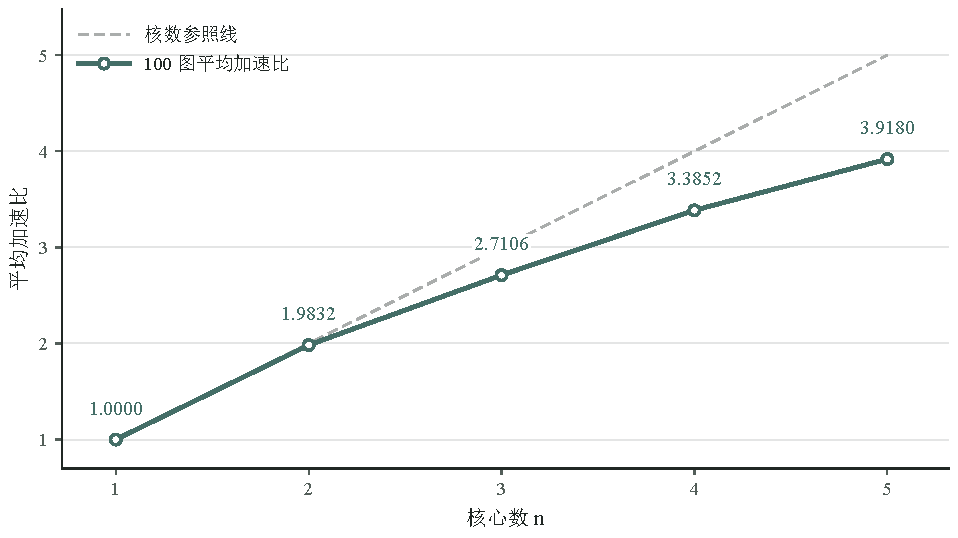
\includegraphics[width=.90\textwidth]{../求解/问题一/图片/q1_mean.pdf}
\caption{第一问各核数平均加速比}\label{fig:q1_mean}\end{figure}

\subsubsection{逐例分布及低收益图}
图~\ref{fig:q1_distribution} 展示二至五核加速比的经验分布。五核配置下，100 个图的加速比介于 $1.5157$ 与 $6.3928$，其中 6 个图低于 2，9 个图超过 5。均值低于中位数，说明少数低收益图对总体平均值有明显影响。
\begin{figure}[htbp]\centering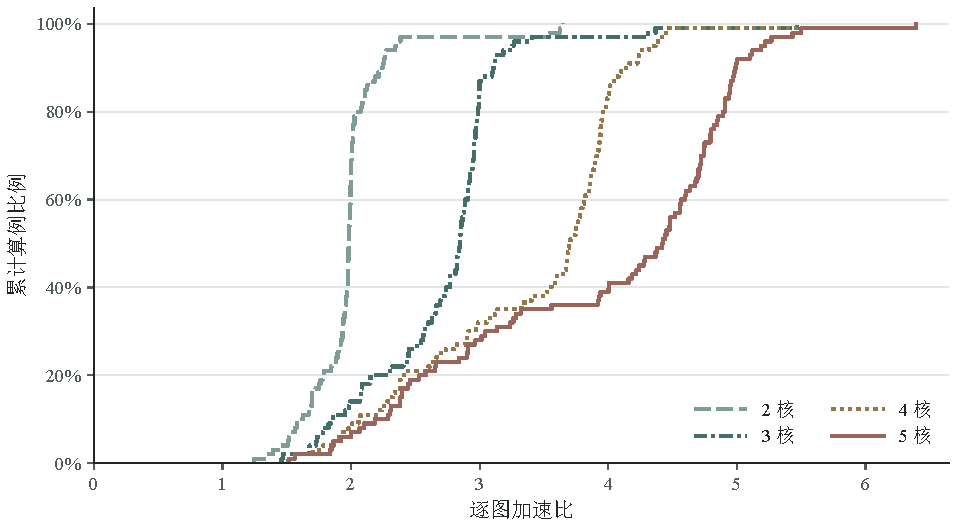
\includegraphics[width=.90\textwidth]{../求解/问题一/图片/q1_distribution.pdf}
\caption{第一问各核数加速比的逐例分布}\label{fig:q1_distribution}\end{figure}

与原始整图单核参考相比，多核方案还调整了分组和执行顺序，并可能改变自动换出与流水线重叠。该比较不只改变核心数，所以 $S=n$ 是参照线，加速比可以超过这一数值。低收益算例则需要结合计算依赖链、任务边界、负载分配和搬运争用分析。

本问五核额外 COPY 字节的均值为 $14585335.66$ B，中位数为 $1990466$ B，差异说明搬运规模具有明显长尾。88 个五核结果未产生自动换出的额外 COPY，其余12个结果呈现片上存储压力。

\subsubsection{任意时刻可用解与搜索过程}
搜索从同配置的已有可行方案或本次构造的初始候选出发。以下轨迹记录本次运行中完成评价和保存后可用的方案，不包含已有方案在此前运行中的生成用时；本次保存耗时计入可用时刻，跨过采点后才可用的解只进入后续采点。设 $\tau$ 为本次运行累计用时，$\mathcal A(\tau)$ 为在该时刻前已经完整评价并保存的可用候选集合。当该集合非空时，定义
\begin{equation}
 U(\tau)=\min_{x\in\mathcal A(\tau)}C_q(x).
 \label{eq:anytime}
\end{equation}
图~\ref{fig:q1_anytime} 以100个算例编号为纵轴、运行用时（秒）为横轴，每30秒采点。对算例 $i$，颜色表示当前可用周期相对最终周期的超额比例 $U_i(\tau)/C_{i,1,5}-1$，为无量纲量。30秒时93个算例取得可用解，其余位置留空。停止后若无新可用解，$U_i(\tau)$ 保持不变。
\begin{figure}[htbp]\centering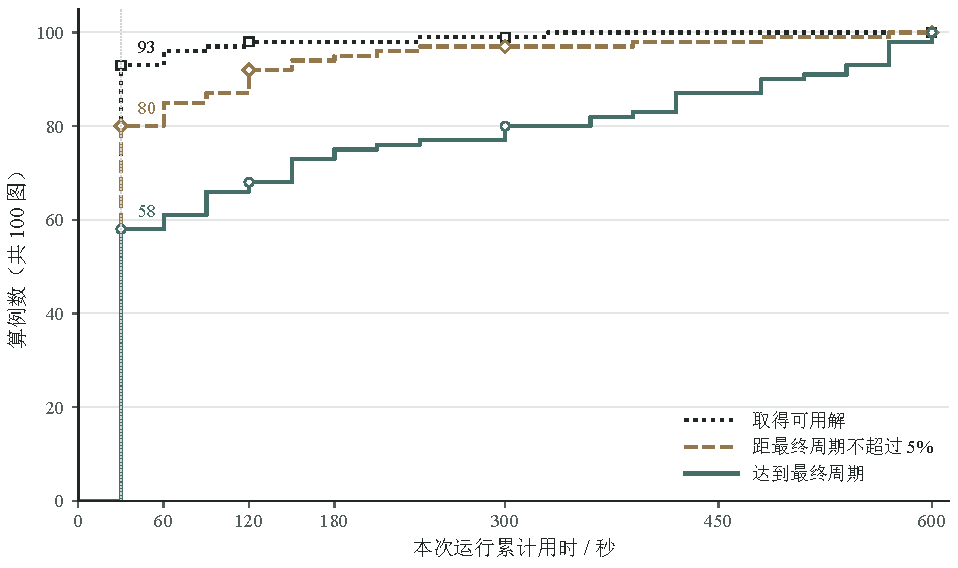
\includegraphics[width=\textwidth]{../求解/问题一/图片/q1_anytime.pdf}
\caption{第一问五核可用解的相对周期差距}\label{fig:q1_anytime}\end{figure}

\subsubsection{下界与结果解释}
图~\ref{fig:q1_bound} 对照五核结果周期及全局下界。下界接近结果时，继续搜索能够带来的相对周期减少受到式~\eqref{eq:gap} 约束；下界较松时，差距同时受方案质量和松弛程度影响，任务交接、容量与带宽竞争等未被充分刻画的约束也可能扩大该区间。
\begin{figure}[H]\centering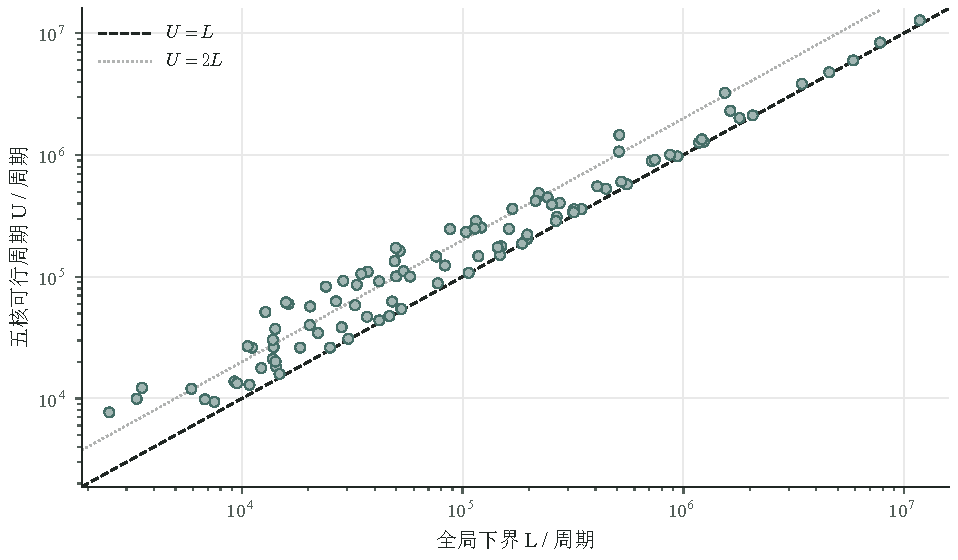
\includegraphics[width=.92\textwidth]{../求解/问题一/图片/q1_bound.pdf}
\caption{第一问五核可行周期与全局下界}\label{fig:q1_bound}\end{figure}

在这100个算例上，联合划分与调度取得了上述多核结果。第二问沿用决策和接受准则，将任务边界扩展到核心，考察同核片上驻留和跨核交接的变化。
